\chapter{Het hart en de hartcyclus}\label{ch:b2:heart}

Snijd het \omterm{def:b2:heart:anatomy}{hart} uit een kikker, leg het in een zoutoplossing, en het blijft
urenlang kloppen --- geen zenuwen, geen hersenen, geen \omterm{def:b2:blood-circulation:blood}{bloed}, alleen een
spier die ongeveer eens per seconde uit zichzelf samentrekt omdat een
klein plekje van zijn cellen niet stil kan blijven. Een menselijk \omterm{def:b2:heart:anatomy}{hart} doet
dit in een leven zo'n drie miljard keer en verplaatst in de orde van
tweehonderd miljoen liter, zonder ooit te worden uitgeschakeld. Dit
hoofdstuk gaat over die pomp: zijn holten en kleppen, de cyclus van vullen
en legen en de drukken die hem aandrijven, het elektrische systeem dat hem
timet en het spoor dat het op de huid achterlaat, de wet die hem zijn
debiet slag voor slag laat afstemmen op zijn instroom, en de zenuwen en
hormonen die zijn tempo en kracht bijstellen.

\section{De pomp}

\begin{definition}[Holten en kleppen]\label{def:b2:heart:anatomy}
\index{hart}\index{atrium}\index{ventrikel}\index{hartklep}
Het hart bestaat uit twee pompen naast elkaar, elk een \emph{atrium} dat
\omterm{def:b2:blood-circulation:blood}{bloed} uit de \omterm{def:b2:blood-circulation:vessels}{aders} ontvangt en een \emph{ventrikel} dat het in een \omterm{def:b2:blood-circulation:vessels}{slagader}
uitstoot. Het rechterhart krijgt \omterm{def:b2:blood-circulation:blood}{bloed} uit de holle \omterm{def:b2:blood-circulation:vessels}{aders} en stuurt het via
de longslagader naar de longen; het linkerhart krijgt het via de longaders
terug en stuurt het via de aorta rond het lichaam. Vier kleppen maken de
stroming eenrichtingsverkeer: de \emph{atrioventriculaire kleppen}
(tricuspidalisklep rechts, mitralisklep links), slippen die met peesdraden
aan papillairspieren vastzitten, zodat ze niet in het atrium kunnen
terugslaan; en de \emph{halvemaanvormige kleppen} (pulmonalis- en
aortaklep), drie zakjes die zich vullen en afsluiten wanneer de arteriële
druk die van het ventrikel overtreft. De kleppen zijn passief: ze gaan
alleen op drukverschillen open en dicht. De ventrikelwand is
\emph{myocard}, dwarsgestreepte spier uit vertakte cellen die kop aan staart
zijn verbonden door \emph{intercalaire schijven} vol gap junctions, zodat
het hele ventrikel elektrisch één cel is en als één geheel samentrekt; de
wand van het linkerventrikel is drie keer zo dik als die van het rechter,
omdat het tegen vijf keer zo hoge druk pompt. De hartspier wordt gevoed door
eigen \emph{kransslagaders}, die zich in de diastole vullen, en draait
vrijwel volledig op aeroob metabolisme --- hij kan niet lenen.
\end{definition}

\begin{omfigure}
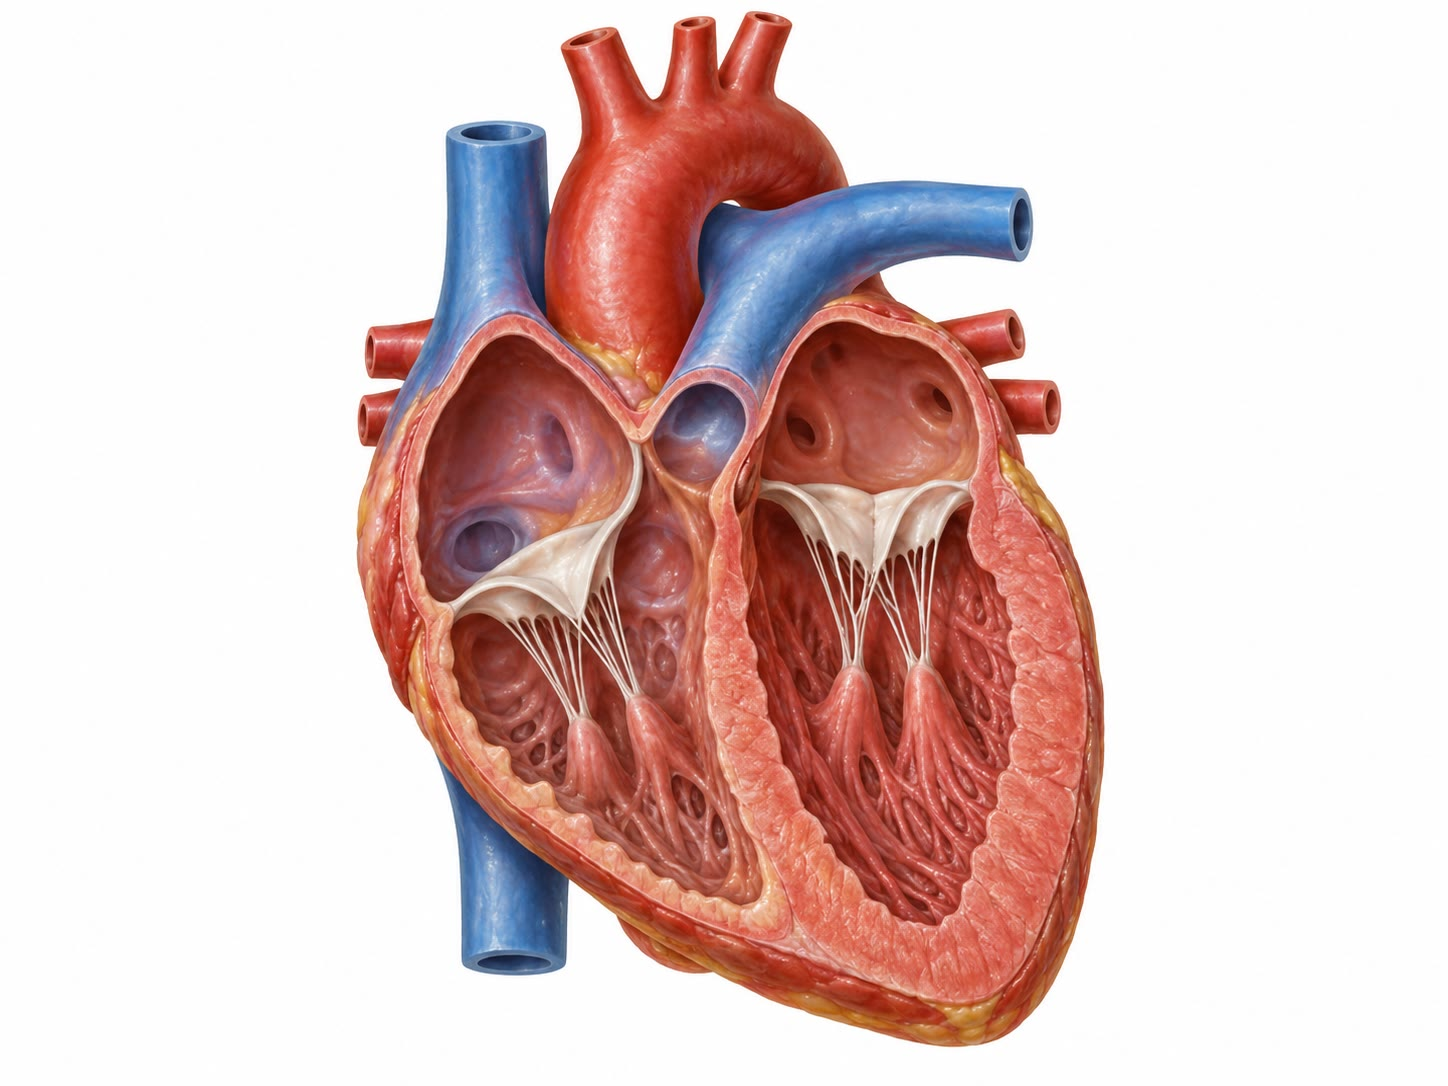
\includegraphics[width=0.55\linewidth]{images/book4/ai/b4-17-heart-cutaway.jpg}

{\small Het \omterm{def:b2:heart:anatomy}{hart} in frontale doorsnede: twee atria boven, twee \omterm{def:b2:heart:anatomy}{ventrikels}
onder, het dikke linkerventrikel, de atrioventriculaire kleppen met hun
peesdraden, en de twee grote \omterm{def:b2:blood-circulation:vessels}{slagaders} die bovenaan vertrekken.}
\end{omfigure}

\begin{proposition}[De hartcyclus]\label{prop:b2:heart:cycle}
\index{hartcyclus}\index{systole}\index{diastole}\index{slagvolume}\index{ejectiefractie}
Eén slag duurt in rust ongeveer \qty{0.8}{s}. \emph{Diastole}
(\qty{0.5}{s}): de \omterm{def:b2:heart:anatomy}{ventrikels} ontspannen, hun druk zakt onder die van de
atria, de atrioventriculaire kleppen gaan open en \omterm{def:b2:blood-circulation:blood}{bloed} stroomt binnen,
grotendeels passief, en daarna met een laatste duw van de samentrekking van
de atria; aan het eind van de diastole bevat het \omterm{def:b2:heart:anatomy}{ventrikel} ongeveer
\qty{120}{mL} (het \emph{einddiastolisch volume}). \emph{Systole}
(\qty{0.3}{s}): de \omterm{def:b2:heart:anatomy}{ventrikels} trekken samen; zodra hun druk die van de atria
overtreft, sluiten de atrioventriculaire kleppen (de eerste harttoon,
``boem''), en enkele honderdsten van een seconde knijpt het \omterm{def:b2:heart:anatomy}{ventrikel} een
gesloten holte samen --- \emph{isovolumetrische contractie} ---
tot zijn druk de arteriële druk passeert (\qty{80}{mmHg} links), waarna de
halvemaanvormige kleppen opengaan en \omterm{def:b2:blood-circulation:blood}{bloed} wordt uitgestoten. Het
linkerventrikel bereikt \qty{120}{mmHg} en stoot ongeveer
\qty{70}{mL} uit (het \emph{\omterm{prop:b2:heart:cycle}{slagvolume}}, een \emph{\omterm{prop:b2:heart:cycle}{ejectiefractie}}
van \qty{60}{\%}); terwijl het ontspant, zakt zijn druk onder die van de
aorta, slaat de aortaklep dicht (de tweede toon, ``tak''), en brengt een
isovolumetrische relaxatie de druk terug tot het niveau van het \omterm{def:b2:heart:anatomy}{atrium},
waarna het vullen weer begint. Het rechterhart doet hetzelfde bij een
vijfde van de druk en stoot hetzelfde volume uit.
\end{proposition}

\begin{omfigure}
\begin{tikzpicture}
\begin{axis}[
  width=0.9\linewidth, height=7.2cm,
  axis x line=bottom, axis y line=left,
  xmin=0, xmax=0.8, ymin=0, ymax=130,
  xlabel={tijd in de cyclus (s)}, ylabel={druk (\unit{mmHg})},
  xlabel style={font=\small, at={(axis description cs:0.5,-0.1)}, anchor=north},
  ylabel style={font=\small},
  tick label style={font=\small}, xtick={0,0.1,0.3,0.8}, ytick={0,40,80,120},
  legend style={font=\scriptsize, at={(0.6,0.45)}, anchor=west, draw=none},
  clip=false,
]
% aortic pressure
\addplot[very thick, omThm] coordinates {(0,82) (0.05,80) (0.1,80) (0.12,95) (0.16,115) (0.2,120) (0.25,112) (0.3,100) (0.32,104) (0.34,100) (0.45,94) (0.6,88) (0.8,82)};
\addlegendentry{aorta}
% left ventricular pressure
\addplot[very thick, omDef] coordinates {(0,5) (0.04,8) (0.05,10) (0.08,60) (0.1,80) (0.12,95) (0.16,115) (0.2,120) (0.25,112) (0.3,100) (0.32,60) (0.35,20) (0.38,5) (0.5,3) (0.7,5) (0.75,8) (0.8,5)};
\addlegendentry{linkerventrikel}
% atrial pressure
\addplot[thick, omProp] coordinates {(0,6) (0.03,9) (0.06,6) (0.1,8) (0.15,6) (0.3,7) (0.36,10) (0.4,5) (0.6,6) (0.75,9) (0.8,6)};
\addlegendentry{linkeratrium}
\draw[dashed, gray] (axis cs:0.05,0) -- (axis cs:0.05,128); \node[font=\scriptsize, anchor=south, align=center] at (axis cs:0.05,128) {mitralis\\sluit};
\draw[dashed, gray] (axis cs:0.1,0) -- (axis cs:0.1,128); \node[font=\scriptsize, anchor=south, align=center] at (axis cs:0.13,128) {aortaklep\\opent};
\draw[dashed, gray] (axis cs:0.31,0) -- (axis cs:0.31,128); \node[font=\scriptsize, anchor=south, align=center] at (axis cs:0.31,128) {aortaklep\\sluit};
\draw[dashed, gray] (axis cs:0.38,0) -- (axis cs:0.38,128); \node[font=\scriptsize, anchor=south, align=center] at (axis cs:0.4,128) {mitralis\\opent};
\node[font=\scriptsize] at (axis cs:0.2,45) {systole};
\node[font=\scriptsize] at (axis cs:0.55,25) {diastole};
\end{axis}
\end{tikzpicture}

{\small Drukken in het linkerhart gedurende één slag. Het \omterm{def:b2:heart:anatomy}{ventrikel} knijpt
een gesloten holte samen tot het de aortadruk overtreft, stoot uit zolang
het erboven blijft, ontspant tot zijn druk onder die van het \omterm{def:b2:heart:anatomy}{atrium} zakt, en
vult zich.}
\end{omfigure}

\begin{theorem}[De arbeid van het hart]\label{thm:b2:heart:work}
\index{hartarbeid}\index{druk-volumelus}
Uitgezet als druk tegen volume beschrijft één slag van het linkerventrikel
een lus --- vullen langs de onderkant, isovolumetrische contractie langs de
rechterkant omhoog, uitstoting langs de bovenkant van
\qty{120}{mL} tot \qty{50}{mL}, isovolumetrische relaxatie langs de
linkerkant omlaag --- en de oppervlakte van de lus is de mechanische arbeid
van de slag:
\[
W = \oint P\,\mathrm{d}V \approx \bar P_{\text{uitstoting}}\times \text{slagvolume} \approx \qty{100}{mmHg}\times\qty{70}{mL} = \qty{0.93}{J}.
\]
Bij 72 slagen per minuut levert het linkerventrikel ongeveer \qty{1.1}{W},
het rechter \qty{0.2}{W}; het metabolisme van het \omterm{def:b2:heart:anatomy}{hart} bedraagt zo'n
\qty{8}{W}, zodat zijn mechanisch rendement bij \qty{15}{\%} ligt, en de rest
warmte en de kosten van spanning zijn. Verhoging van de druk waartegen het
\omterm{def:b2:heart:anatomy}{hart} pompt (hypertensie, een vernauwde aortaklep) verhoogt de arbeid per
slag evenredig, en de spier verdikt zich als reactie, zoals elke spier ---
tot zijn kransslagaderlijke aanvoer zijn omvang niet meer kan bijhouden.
\end{theorem}
\begin{proof}
Arbeid is kracht maal afstand, en voor een druk die op een bewegende wand
werkt, druk maal doorlopen volume: $\mathrm{d}W = P\,\mathrm{d}V$.
Over een gesloten lus is de netto arbeid de ingesloten oppervlakte (vullen
bij lage druk kost weinig; uitstoten bij hoge druk levert veel meer op).
$\qty{100}{mmHg} = \qty{1.33e4}{Pa}$ en $\qty{70}{mL} =
\qty{7e-5}{m^3}$: $1.33\times 10^{4}\times 7\times 10^{-5} =
\qty{0.93}{J}$; maal $1.2$ slagen per seconde geeft \qty{1.1}{W}.
\end{proof}

\begin{omfigure}
\begin{tikzpicture}
\begin{axis}[
  width=0.62\linewidth, height=6cm,
  axis x line=bottom, axis y line=left,
  xmin=0, xmax=150, ymin=0, ymax=140,
  xlabel={volume van het linkerventrikel (\unit{mL})}, ylabel={druk (\unit{mmHg})},
  xlabel style={font=\small, at={(axis description cs:0.5,-0.12)}, anchor=north},
  ylabel style={font=\small},
  tick label style={font=\small}, xtick={0,50,120}, ytick={0,80,120},
  clip=false,
]
\fill[omDef!12] (axis cs:50,5) -- (axis cs:120,8) -- (axis cs:120,80) -- (axis cs:110,115) -- (axis cs:80,122) -- (axis cs:50,100) -- cycle;
\draw[very thick, omDef, ->] (axis cs:50,5) -- (axis cs:120,8);
\draw[very thick, omDef, ->] (axis cs:120,8) -- (axis cs:120,80);
\draw[very thick, omDef, ->] (axis cs:120,80) .. controls (axis cs:110,118) and (axis cs:80,125) .. (axis cs:50,100);
\draw[very thick, omDef, ->] (axis cs:50,100) -- (axis cs:50,5);
\node[font=\scriptsize, anchor=south] at (axis cs:85,11) {vullen};
\node[font=\scriptsize, anchor=west] at (axis cs:122,44) {isovolumetrische contractie};
\node[font=\scriptsize, anchor=south] at (axis cs:85,124) {uitstoting};
\node[font=\scriptsize, anchor=east] at (axis cs:48,52) {relaxatie};
\node[font=\scriptsize] at (axis cs:85,60) {oppervlakte $=$ arbeid, \qty{0.9}{J}};
\end{axis}
\end{tikzpicture}

{\small De \omterm{thm:b2:heart:work}{druk-volumelus} van het linkerventrikel. De ingesloten
oppervlakte is de arbeid van één slag; een hogere arteriële druk verhoogt
de bovenkant van de lus en daarmee de arbeid.}
\end{omfigure}

\section{De eigen klok van het hart}

\begin{proposition}[Automatie en geleiding]\label{prop:b2:heart:conduction}
\index{sinusknoop}\index{pacemaker}\index{atrioventriculaire knoop}\index{purkinjevezels}
De slag ontstaat in de \emph{sinusknoop}, een plekje gespecialiseerde
spiercellen in de wand van het rechteratrium waarvan de membraanpotentiaal
nooit rust: na elke actiepotentiaal stijgt hij langzaam (een
\emph{pacemakerpotentiaal}, aangedreven door een natriumstroom die bij
negatieve potentialen aanschakelt en door calciumkanalen) tot hij de drempel
bereikt en opnieuw vuurt, ongeveer honderd keer per minuut als hij met rust
wordt gelaten. De impuls verspreidt zich door de spier van de atria, van cel
tot cel via de gap junctions, en de atria trekken samen; hij bereikt de
\emph{\omterm{prop:b2:heart:conduction}{atrioventriculaire knoop}}, de enige elektrische brug tussen atria en
\omterm{def:b2:heart:anatomy}{ventrikels}, die traag geleidt en hem een tiende seconde vertraagt --- tijd
voor de atria om het vullen van de \omterm{def:b2:heart:anatomy}{ventrikels} af te maken; daarna jaagt hij
door de \emph{bundel van His} en de \emph{purkinjevezels}, snel geleidende
cellen die hem binnen \qty{30}{ms} aan de hele ventrikelspier afleveren,
zodat de \omterm{def:b2:heart:anatomy}{ventrikels} van de apex naar boven toe, als één geheel, samentrekken
en het \omterm{def:b2:blood-circulation:blood}{bloed} naar de uitstroomkleppen drijven. Elk deel van dit systeem kan
zelf het ritme aangeven, elk trager dan het vorige (de sinusknoop met 100,
de AV-knoop met 50, de purkinjevezels met 30), zodat bij uitval van de
sinusknoop een lager centrum het overneemt --- in een trager tempo.
\end{proposition}
\begin{proof}[Bewijsmateriaal]
Een geïsoleerd \omterm{def:b2:heart:anatomy}{hart}, of een strookje weefsel uit de sinusknoop, klopt in een
schaaltje zonder zenuwen; een strookje \omterm{def:b2:heart:anatomy}{ventrikel} klopt ook, maar trager. Het
afkoelen of opwarmen van alleen de sinusknoop verandert het tempo van het
hele \omterm{def:b2:heart:anatomy}{hart}; het doorsnijden van de AV-bundel ontkoppelt de \omterm{def:b2:heart:anatomy}{ventrikels}, die dan
in hun eigen trage ritme kloppen terwijl de atria doorgaan in dat van de
sinusknoop (hartblok). Registratie van één enkele cel van de sinusknoop
toont de trage diastolische depolarisatie die geen gewone spiercel heeft;
blokkering van de pacemakerstroom vertraagt haar.
\end{proof}

\begin{omfigure}
\begin{tikzpicture}[every node/.style={font=\scriptsize}, >=stealth]
  % simplified heart outline, scaled up
  \draw[thick, fill=omThm!6] (0,0) .. controls (-4.2,1.3) and (-3.8,5.4) .. (-1.3,5.8) .. controls (0,6.1) and (0.6,5.6) .. (1.3,5.8) .. controls (3.8,5.4) and (4.2,1.3) .. (0,0);
  \draw[thick] (-3.0,3.5) .. controls (-0.8,3.85) and (0.8,3.85) .. (3.0,3.5);
  \draw[thick] (0,3.75) -- (0,0.6);
  \node at (-1.5,4.7) {rechteratrium}; \node at (1.5,4.7) {linkeratrium};
  \node[align=center] at (-1.3,2.55) {rechter-\\ventrikel}; \node[align=center] at (1.3,2.55) {linker-\\ventrikel};
  % SA node
  \fill[omDef] (-2.5,5.0) circle (0.16); \node[omDef, anchor=east] at (-3.3,5.4) {sinusknoop}; \draw[omDef] (-3.3,5.35) -- (-2.62,5.08);
  \draw[omDef, dashed] (-2.5,5.0) circle (0.45); \draw[omDef, dashed] (-2.5,5.0) circle (0.8);
  % AV node
  \fill[omDef] (-0.25,3.7) circle (0.14); \node[omDef, anchor=west] at (0.15,4.05) {AV-knoop}; \draw[omDef] (0.15,4.05) -- (-0.12,3.78);
  % bundle and Purkinje
  \draw[very thick, omDef] (-0.25,3.6) -- (-0.25,2.1);
  \draw[very thick, omDef] (-0.25,2.1) .. controls (-0.8,1.4) .. (-1.9,1.1);
  \draw[very thick, omDef] (-0.25,2.1) .. controls (0.8,1.4) .. (1.9,1.1);
  \foreach \p in {(-1.9,1.1),(1.9,1.1)} { \draw[omDef] \p -- ++(-0.3,0.6); \draw[omDef] \p -- ++(0.3,0.7); \draw[omDef] \p -- ++(0,0.85); }
  \node[omDef, anchor=west] at (3.4,1.0) {purkinjevezels}; \draw[omDef] (3.4,1.0) -- (2.2,1.1);
  \node[omDef, anchor=east] at (-0.45,3.05) {bundel van His};
  % timing
  \node[anchor=west, align=left] at (5.6,5.0) {sinusknoop vuurt: $t = 0$\\atria depolariseren: 0--\qty{80}{ms}};
  \node[anchor=west, align=left] at (5.6,3.5) {vertraging in de AV-knoop: \qty{100}{ms}};
  \node[anchor=west, align=left] at (5.6,1.9) {bundel en purkinjevezels:\\ventrikels gedepolariseerd\\na \qty{220}{ms}, apex eerst};
\end{tikzpicture}

{\small Het geleidingssysteem. De sinusknoop vuurt, de atria depolariseren,
de \omterm{prop:b2:heart:conduction}{atrioventriculaire knoop} vertraagt de impuls, en de bundel en de
purkinjevezels leveren hem van de apex naar boven toe aan de \omterm{def:b2:heart:anatomy}{ventrikels} af.}
\end{omfigure}

\begin{proposition}[Het elektrocardiogram]\label{prop:b2:heart:ecg}
\index{elektrocardiogram}
Het \omterm{def:b2:heart:anatomy}{hart} is een grote massa cellen die na elkaar depolariseren en
repolariseren, en de stromen die in het lichaam eromheen lopen, kunnen tussen
elektroden op de ledematen worden geregistreerd als spanningen van een
millivolt: het \emph{elektrocardiogram}. Zijn golven zijn de gebeurtenissen
van het geleidingssysteem: de \emph{P-golf} is de depolarisatie van de atria;
het vlakke \emph{PR-interval} (\qty{0.16}{s}) is de AV-vertraging; het
\emph{QRS-complex}, scherp en kort (\qty{0.08}{s}), is de depolarisatie van
de \omterm{def:b2:heart:anatomy}{ventrikels} --- groot omdat de ventrikelmassa groot is, kort omdat de
purkinjevezels snel zijn; de \emph{T-golf} is de repolarisatie van de
\omterm{def:b2:heart:anatomy}{ventrikels}. (De repolarisatie van de atria gaat verloren in het QRS.) Het
spoor meldt timing en geleiding, geen kracht: een geblokkeerde AV-knoop
verlengt het PR-interval of ontkoppelt P van QRS, een afgestorven gebied van
het \omterm{def:b2:heart:anatomy}{ventrikel} vervormt het QRS, een onregelmatig \omterm{def:b2:heart:anatomy}{atrium}
(boezemfibrilleren) vervangt de P-golven door ruis en laat de \omterm{def:b2:heart:anatomy}{ventrikels}
onregelmatig kloppen, en een interval tussen R-toppen geeft het tempo.
\end{proposition}

\begin{omfigure}
\begin{tikzpicture}
\begin{axis}[
  width=0.9\linewidth, height=5.2cm,
  axis x line=bottom, axis y line=left,
  xmin=0, xmax=1.0, ymin=-0.4, ymax=1.3,
  xlabel={tijd (s)}, ylabel={mV},
  xlabel style={font=\small, at={(axis description cs:0.5,-0.12)}, anchor=north},
  ylabel style={font=\small},
  tick label style={font=\small}, xtick={0,0.2,0.4,0.6,0.8,1.0}, ytick={0,1},
  clip=false,
]
\addplot[very thick, omDef] coordinates {(0,0) (0.08,0) (0.1,0.05) (0.14,0.15) (0.18,0.05) (0.2,0) (0.28,0) (0.3,-0.1) (0.31,0) (0.33,1.1) (0.35,0) (0.36,-0.25) (0.375,0) (0.5,0) (0.54,0.1) (0.58,0.28) (0.62,0.1) (0.65,0) (0.88,0) (0.9,0.05) (0.94,0.15) (0.98,0.05) (1.0,0)};
\node[font=\scriptsize, anchor=south] at (axis cs:0.14,0.17) {P};
\node[font=\scriptsize, anchor=south] at (axis cs:0.33,1.12) {R};
\node[font=\scriptsize, anchor=north] at (axis cs:0.295,-0.11) {Q};
\node[font=\scriptsize, anchor=north] at (axis cs:0.365,-0.27) {S};
\node[font=\scriptsize, anchor=south] at (axis cs:0.58,0.3) {T};
\draw[<->, gray] (axis cs:0.1,0.45) -- (axis cs:0.3,0.45); \node[font=\scriptsize, anchor=south, gray] at (axis cs:0.2,0.46) {PR \qty{0.16}{s}};
\draw[<->, gray] (axis cs:0.3,0.6) -- (axis cs:0.375,0.6); \node[font=\scriptsize, anchor=west, gray] at (axis cs:0.38,0.6) {QRS \qty{0.08}{s}};
\draw[<->, gray] (axis cs:0.33,1.25) -- (axis cs:0.94,1.25); \node[font=\scriptsize, anchor=south, gray] at (axis cs:0.63,1.25) {R-R-interval $=$ 60/frequentie};
\end{axis}
\end{tikzpicture}

{\small Een normaal elektrocardiogram: P (atria), de PR-vertraging in de
AV-knoop, QRS (depolarisatie van de \omterm{def:b2:heart:anatomy}{ventrikels}), T (repolarisatie van de
\omterm{def:b2:heart:anatomy}{ventrikels}).}
\end{omfigure}

\section{Het debiet regelen}

\begin{theorem}[De wet van Frank--Starling]\label{thm:b2:heart:starling}
\index{wet van Frank--Starling}\index{voorbelasting}\index{hartminuutvolume}
De kracht van een ventrikelcontractie stijgt met het volume waarmee het is
gevuld: binnen het werkbereik stoot het \omterm{def:b2:heart:anatomy}{ventrikel} in de systole meer uit
naarmate het in de diastole meer is opgerekt (de \emph{voorbelasting}). Het
\omterm{def:b2:heart:anatomy}{hart} pompt dus slag voor slag uit wat het ontvangt --- een stijging van de
veneuze terugvloed met \qty{20}{\%} wordt beantwoord met een stijging van
het \omterm{prop:b2:heart:cycle}{slagvolume} met \qty{20}{\%}, zonder enige zenuw of enig hormoon --- en
de twee \omterm{def:b2:heart:anatomy}{ventrikels}, die hetzelfde volume moeten verplaatsen, houden elkaar
automatisch in evenwicht: als het rechterhart meer \omterm{def:b2:blood-circulation:blood}{bloed} naar de longen
stuurt, ontvangt het linkerhart meer en pompt het meer. Het mechanisme zit
in het \omterm{def:b2:cell-differentiation:fibre}{sarcomeer}: bij de korte lengten van een slecht gevuld \omterm{def:b2:heart:anatomy}{ventrikel}
overlappen de dikke en dunne filamenten te veel en is de gevoeligheid voor
calcium laag; oprekken naar de optimale lengte
(\qty{2.2}{\micro m}) vergroot zowel de overlapping die voor
dwarsbruggen beschikbaar is als de gevoeligheid, zodat dezelfde calciumpuls
meer kracht oplevert. Voorbij het optimum (een overrekt, falend \omterm{def:b2:heart:anatomy}{hart}) daalt
de kracht weer.
\end{theorem}
\begin{proof}[Bewijsmateriaal]
Frank (1895) registreerde de druk die een kikkerventrikel ontwikkelde bij
vulling met verschillende volumes: de piekdruk steeg met het vulvolume tot
een maximum en daalde daarna. Starling (1914) toonde met een
hart-longpreparaat van een hond, waarin veneuze terugvloed en arteriële
weerstand onafhankelijk konden worden ingesteld, aan dat een grotere
terugvloed het debiet slag voor slag verhoogde, en dat een hogere arteriële
weerstand na enkele slagen van ophoping werd beantwoord met een groter
einddiastolisch volume en een hersteld debiet --- het \omterm{def:b2:heart:anatomy}{ventrikel} beantwoordt
een belasting met rekken en een rek met krachtiger samentrekken.
\end{proof}

\begin{omfigure}
\begin{tikzpicture}
\begin{axis}[
  width=0.66\linewidth, height=5.4cm,
  axis x line=bottom, axis y line=left,
  xmin=0, xmax=200, ymin=0, ymax=140,
  xlabel={einddiastolisch volume (\unit{mL})}, ylabel={slagvolume (\unit{mL})},
  xlabel style={font=\small, at={(axis description cs:0.5,-0.13)}, anchor=north},
  ylabel style={font=\small},
  tick label style={font=\small}, xtick={0,50,100,150,200}, ytick={0,50,100},
  legend style={font=\scriptsize, at={(0.5,-0.3)}, anchor=north, draw=none, legend columns=3},
  clip=false,
]
\addplot[very thick, omDef, domain=40:200, samples=60] {130*(1-exp(-(x-40)/70))};
\addlegendentry{normaal}
\addplot[very thick, omThm, domain=40:200, samples=60] {130*1.3*(1-exp(-(x-40)/55))};
\addlegendentry{met sympathische stimulatie}
\addplot[very thick, omExo!70!black, domain=40:200, samples=60] {130*0.5*(1-exp(-(x-40)/90))};
\addlegendentry{falend hart}
\fill[omDef] (axis cs:120,88) circle (2pt); \node[font=\scriptsize, anchor=south east] at (axis cs:118,90) {rust};
\end{axis}
\end{tikzpicture}

{\small Curven van Starling. Het \omterm{prop:b2:heart:cycle}{slagvolume} stijgt met de vulling; de
sympathische zenuwen verschuiven de curve omhoog (meer debiet bij dezelfde
vulling), een falend \omterm{def:b2:heart:anatomy}{hart} verschuift haar omlaag.}
\end{omfigure}

\begin{proposition}[Zenuwen en hormonen]\label{prop:b2:heart:control}
\index{sympathisch zenuwstelsel!hart}\index{nervus vagus}\index{adrenaline}\index{hartminuutvolume}
Het hartminuutvolume is hartfrequentie maal \omterm{prop:b2:heart:cycle}{slagvolume}, \qty{5}{L/min}
in rust en tot \qty{25}{L/min} bij inspanning van een getrainde atleet.
Beide factoren worden door de autonome zenuwen bepaald. De \emph{\omterm{prop:b2:heart:control}{nervus
vagus}} (parasympathisch), die acetylcholine op de sinusknoop afgeeft,
vertraagt de pacemakerstijging en houdt de rustfrequentie op 70 in plaats
van de eigen 100 van de sinusknoop; snijd de vagi door en de frequentie
stijgt. De \emph{sympathische} zenuwen, die noradrenaline afgeven, en het
bijniermerg, dat \emph{adrenaline} in het \omterm{def:b2:blood-circulation:blood}{bloed} afgeeft, versnellen de
stijging (meer slagen), versnellen de geleiding, en verhogen de
contractiekracht bij elke vulling (een steilere curve van Starling, de
eigenschap die \emph{contractiliteit} heet), door het calcium te verhogen
dat bij elke slag aan de sarcomeren wordt geleverd. Bij inspanning wordt
eerst de vagale rem losgelaten en daarna het sympathische gaspedaal
ingedrukt, en een frequentie van 180 met een \omterm{prop:b2:heart:cycle}{slagvolume} van \qty{140}{mL}
geeft \qty{25}{L/min}; de signalen worden doorgegeven via de receptoren en
secundaire boodschappers van \cref{ch:b2:cell-signalling}, en het geheel
wordt aangestuurd door de drukregelende centra van
\cref{ch:b2:blood-pressure}.
\end{proposition}

\begin{example}[Een hart lezen]\label{ex:b2:heart:reading}
Twee tonen per slag: boem, de AV-kleppen die aan het begin van de systole
sluiten; tak, de halvemaanvormige kleppen die aan het eind ervan sluiten.
Een hartgeruis is turbulente stroming door een vernauwde klep (een stenose)
of terug door een lekkende (een insufficiëntie): een geruis tussen boem en
tak is een lekkende mitralisklep of een vernauwde aortaklep, na tak een
lekkende aortaklep. Een pols van 70 met een bloeddruk van
$120/80$~mmHg betekent een \omterm{prop:b2:heart:cycle}{slagvolume} van ongeveer \qty{70}{mL};
een frequentie van 40 bij een atleet is een groot \omterm{prop:b2:heart:cycle}{slagvolume} en een sterke
vagale tonus; een frequentie van 40 met een PR-interval dat langer wordt tot
er een slag uitvalt, is een zieke AV-knoop. De fysiologie van dit hoofdstuk
is wat een arts in dertig seconden met een stethoscoop hoort.
\end{example}

\section{Opgaven}

\begin{exercise}[$\star$]\label{exo:b2:heart:1}
Volg een druppel \omterm{def:b2:blood-circulation:blood}{bloed} van de holle \omterm{def:b2:blood-circulation:vessels}{ader} tot de aorta, met in volgorde elke
holte, klep en elk vat.
\end{exercise}

\begin{exercise}[$\star$]\label{exo:b2:heart:2}
Geef de fasen van de \omterm{prop:b2:heart:cycle}{hartcyclus} met de toestand van elke klep in elke fase,
en de gebeurtenis die elk van de twee harttonen veroorzaakt.
\end{exercise}

\begin{exercise}[$\star$]\label{exo:b2:heart:3}
Noem de delen van het geleidingssysteem in volgorde, met de tijd die de
impuls nodig heeft om elk deel te bereiken, en de ECG-golf die elk deel
voortbrengt.
\end{exercise}

\begin{exercise}[$\star$]\label{exo:b2:heart:4}
Formuleer de \omterm{thm:b2:heart:starling}{wet van Frank--Starling} en zeg waarom ze garandeert dat de twee
\omterm{def:b2:heart:anatomy}{ventrikels} hetzelfde volume pompen.
\end{exercise}

\begin{exercise}[$\star\star$]\label{exo:b2:heart:5}
Een \omterm{def:b2:heart:anatomy}{hart} heeft een einddiastolisch volume van \qty{130}{mL} en een
eindsystolisch volume van \qty{50}{mL} bij 70 slagen per minuut. Bereken het
\omterm{prop:b2:heart:cycle}{slagvolume}, de \omterm{prop:b2:heart:cycle}{ejectiefractie} en het hartminuutvolume. Een falend \omterm{def:b2:heart:anatomy}{hart} heeft
\qty{180}{mL} en \qty{120}{mL}: bereken opnieuw, en zeg wat er met de
\omterm{prop:b2:heart:cycle}{ejectiefractie} is gebeurd.
\end{exercise}

\begin{exercise}[$\star\star$]\label{exo:b2:heart:6}
Bereken de arbeid van een slag voor een \omterm{prop:b2:heart:cycle}{slagvolume} van \qty{70}{mL} bij een
gemiddelde uitstootdruk van \qty{100}{mmHg}, en het vermogen bij 72 slagen
per minuut. Bereken het opnieuw voor iemand met hypertensie bij
\qty{150}{mmHg}. Hoeveel extra zuurstof per minuut heeft het tweede \omterm{def:b2:heart:anatomy}{hart}
nodig, als het mechanisch rendement \qty{15}{\%} is en \qty{1}{mL} zuurstof
\qty{20}{J} oplevert?
\end{exercise}

\begin{exercise}[$\star\star$]\label{exo:b2:heart:7}
Op een ECG liggen de R-toppen in de ene registratie \qty{0.5}{s} uit elkaar
en in een andere \qty{1.5}{s}. Geef de hartfrequenties. In een derde komen
P-golven om de \qty{0.6}{s} en QRS-complexen om de \qty{1.8}{s}, zonder vast
verband. Wat is er gebeurd?
\end{exercise}

\begin{exercise}[$\star\star$]\label{exo:b2:heart:8}
De potentiaal van een cel van de sinusknoop stijgt vóór elke actiepotentiaal
van \qty{0.15}{s} van \qty{-60}{mV} tot een drempel van \qty{-40}{mV} met
\qty{25}{mV/s}. Bereken het interval tussen de slagen en de frequentie.
Acetylcholine verlaagt de stijging tot \qty{18}{mV/s} en de beginpotentiaal
tot \qty{-65}{mV}; noradrenaline verhoogt de stijging tot
\qty{40}{mV/s}. Bereken beide frequenties.
\end{exercise}

\begin{exercise}[$\star\star$]\label{exo:b2:heart:9}
Leg uit waarom de vertraging in de AV-knoop nodig is, wat er zonder haar met
het debiet zou gebeuren, en waarom een trage AV-knoop (een lang PR-interval)
tot op zekere hoogte onschuldig is en daarboven gevaarlijk.
\end{exercise}

\begin{exercise}[$\star\star\star$]\label{exo:b2:heart:10}
Een atleet heeft in rust een frequentie van 45 en een debiet van
\qty{5}{L/min}; bij inspanning een frequentie van 180 en \qty{30}{L/min}.
Bereken de \omterm{prop:b2:heart:cycle}{slagvolumes} en zeg wat de curve van Starling en de sympathische
zenuwen elk bijdragen. Waarom kan de frequentie niet zinvol boven ongeveer
200 uitkomen?
\end{exercise}

\begin{exercise}[$\star\star\star$]\label{exo:b2:heart:11}
Een vernauwde aortaklep laat een opening van \qty{1}{cm^2} over in plaats van
\qty{3}{cm^2}. Bereken met de continuïteit de snelheid van het uitgestoten
\omterm{def:b2:blood-circulation:blood}{bloed} bij \qty{250}{mL/s} door elk van beide, en, met Bernoulli
($\Delta P = \tfrac12\rho v^2$), de druk die het \omterm{def:b2:heart:anatomy}{ventrikel} in elk geval boven
de aortadruk moet opbrengen. Wat doet het \omterm{def:b2:heart:anatomy}{ventrikel} eraan, en wat zijn de
uiteindelijke kosten?
\end{exercise}

\begin{exercise}[$\star\star\star$]\label{exo:b2:heart:12}
``Het \omterm{def:b2:heart:anatomy}{hart} is een pomp die zichzelf regelt en door het zenuwstelsel alleen
wordt bijgesteld.'' Bespreek dit, met onderscheid tussen wat de automatie,
de \omterm{thm:b2:heart:starling}{wet van Frank--Starling} en de autonome zenuwen elk leveren, en wat een
getransplanteerd \omterm{def:b2:heart:anatomy}{hart} --- dat geen zenuwen heeft --- wel en niet kan.
\end{exercise}

\section{Vraagstuk: een hart onder belasting}

\begin{problem}[{Weekendvraagstuk --- één hart gevolgd van rust tot
inspanning en tot ziekte: zijn cyclus getimed, zijn arbeid berekend, zijn
elektrocardiogram gelezen, zijn Starlingrespons en zijn autonome regeling
gekwantificeerd, en de kosten van een vernauwde klep geschat, met als
besluit het debiet in rust en bij inspanning, de arbeid per slag, en de
gradiënt over de stenose}]
\label{pb:b2:heart:1}
Gegevens: in rust frequentie 70, einddiastolisch volume \qty{130}{mL},
eindsystolisch \qty{60}{mL}, gemiddelde uitstootdruk \qty{100}{mmHg}
($\qty{1}{mmHg} = \qty{133}{Pa}$), aortadruk $120/80$~mmHg.
De systole duurt bij elke frequentie \qty{0.3}{s}. Pacemaker: stijging van
\qty{-60}{mV} tot \qty{-40}{mV}, actiepotentiaal \qty{0.15}{s}. Het
\omterm{def:b2:heart:anatomy}{hart} verbruikt \qty{20}{J} per milliliter zuurstof bij een
mechanisch rendement van \qty{15}{\%}; kransslagaderbloed vervoert
\qty{0.2}{mL} zuurstof per milliliter en het \omterm{def:b2:heart:anatomy}{hart} onttrekt er
\qty{70}{\%} van. Dichtheid van \omterm{def:b2:blood-circulation:blood}{bloed} \qty{1060}{kg/m^3}.

\medskip
\noindent\textbf{Deel I --- De cyclus in rust.}
\begin{enumerate}
  \item Bereken het \omterm{prop:b2:heart:cycle}{slagvolume}, de \omterm{prop:b2:heart:cycle}{ejectiefractie} en het
        hartminuutvolume.
  \item Bereken de duur van één cyclus en van de diastole.
  \item Bereken het gemiddelde uitstootdebiet tijdens de systole, in
        milliliter per seconde, en de gemiddelde snelheid door een aortaklep
        van \qty{3}{cm^2}.
  \item De ventrikeldruk stijgt tijdens de isovolumetrische contractie met
        \qty{1500}{mmHg/s}, van 10 tot \qty{80}{mmHg}. Hoelang duurt die fase?
  \item Bereken de arbeid van één slag en het mechanisch vermogen van het
        linkerventrikel.
  \item Bereken het totale vermogen en het zuurstofverbruik van het \omterm{def:b2:heart:anatomy}{hart}
        (beide \omterm{def:b2:heart:anatomy}{ventrikels}: neem het rechter als een vijfde van het linker).
  \item Bereken de kransslagaderlijke bloedstroom die nodig is om die
        zuurstof te leveren.
\end{enumerate}

\medskip
\noindent\textbf{Deel II --- De pacemaker en het spoor.}
\begin{enumerate}[resume]
  \item Welke stijgsnelheid (\unit{mV/s}) geeft een frequentie van 70?
  \item De \omterm{prop:b2:heart:control}{nervus vagus} wordt doorgesneden: de frequentie wordt 100. Welke
        stijgsnelheid is dat?
  \item Bereken de stijgsnelheid voor een frequentie van 180 bij
        inspanning.
  \item Geef op het ECG in rust het R-R-interval, en zeg waarmee de P-golf,
        het QRS-complex en de T-golf overeenkomen.
  \item Het PR-interval is in rust \qty{0.16}{s}. Zijn lengte is vooral de
        vertraging in de AV-knoop: leg uit wat die vertraging bereikt en
        waarom een frequentie van 180 vereist dat ook de knoop sneller wordt.
  \item Het ECG van een patiënt toont QRS-complexen om de \qty{1.5}{s} en
        P-golven om de \qty{0.8}{s}, zonder verband. Stel de diagnose, geef
        de ventrikelfrequentie, en zeg welk weefsel het ritme van de
        \omterm{def:b2:heart:anatomy}{ventrikels} bepaalt.
\end{enumerate}

\medskip
\noindent\textbf{Deel III --- Inspanning.}
Bij inspanning stijgt de frequentie tot 180 en verhogen de sympathische
zenuwen de contractiliteit, zodat het eindsystolisch volume daalt tot
\qty{30}{mL}; de veneuze terugvloed verhoogt het einddiastolisch volume tot
\qty{150}{mL}.
\begin{enumerate}[resume]
  \item Bereken het \omterm{prop:b2:heart:cycle}{slagvolume}, de \omterm{prop:b2:heart:cycle}{ejectiefractie} en het debiet.
  \item Bereken de duur van de diastole bij 180 en leg uit waarom de
        frequentie niet zinvol veel hoger kan worden.
  \item Bereken het vermogen van het linkerventrikel bij een gemiddelde
        uitstootdruk van \qty{120}{mmHg}, en het zuurstofverbruik van het
        \omterm{def:b2:heart:anatomy}{hart}.
  \item Bereken de nodige kransslagaderlijke bloedstroom, en vergelijk met
        de rust. Waarom is de verkorting van de diastole daarvoor een
        probleem?
  \item Zonder sympathische zenuwen (een getransplanteerd \omterm{def:b2:heart:anatomy}{hart}) stijgt de
        frequentie maar langzaam, via adrenaline in het \omterm{def:b2:blood-circulation:blood}{bloed}, en de
        contractiliteit minder. Voorspel het debiet in de eerste minuut van
        de inspanning, alleen met de wet van Starling en dezelfde vulling.
  \item Verdeel de stijging van het debiet van rust naar inspanning over
        haar drie oorzaken (frequentie, vulling, contractiliteit), in liter
        per minuut elk.
\end{enumerate}

\medskip
\noindent\textbf{Deel IV --- Een vernauwde klep.}
De aortaklep vernauwt tot \qty{1}{cm^2}.
\begin{enumerate}[resume]
  \item Bereken de uitstootsnelheid in rust door de vernauwde klep.
  \item Bereken met Bernoulli, $\Delta P = \tfrac12\rho v^{2}$, de druk die
        het \omterm{def:b2:heart:anatomy}{ventrikel} moet toevoegen om er \omterm{def:b2:blood-circulation:blood}{bloed} door te duwen, in mmHg.
  \item Bereken beide opnieuw bij inspanning.
  \item Wat moet in elk geval de piekdruk van het \omterm{def:b2:heart:anatomy}{ventrikel} zijn om de
        aortadruk normaal te houden, en met welke factor stijgt zijn arbeid
        per slag in rust?
  \item De ventrikelwand verdikt zich als reactie. Leg uit waarom dit helpt
        en waarom het uiteindelijk faalt (denk aan de kransslagaderlijke
        aanvoer en aan de diastolische vulling).
  \item Formuleer het resultaat: het debiet in rust en bij inspanning, de
        arbeid per slag in rust, en de gradiënt over de vernauwde klep in rust
        en bij inspanning.
\end{enumerate}
\end{problem}
